\chapter{交易方案的详细设计和代码实现}



方案的实现设计抽象如下图\ref*{Fig:Design}所示。



实现分为多个层级,最底层为程序设计语言工具链 Golang、数据库 SQLite3 以及全同态加密库 Lattigo;往上一层为共用的内部包(Internal Package),包括定义用户的包 \verb|internal/user|、定义共用数据库操作的包 \verb|internal/db|、定义单笔交易基本信息的包 \verb|internal/transaction|,以及定义密钥的包 \verb|internal/db|;再向上一层则为定义了客户端和服务端主要操作的包 \verb|internal/clientlib,serverlib|。最上层则为本文附带的可能的服务端样例实现。此外,本文亦提供了一些集成测试样例,可以通过 Golang 工具链的测试功能进行运行。对测试的具体描述和结果将放置在下一章描述。

本实现使用了以下第三方包:

\begin{itemize}
    \item \verb|github.com/google/uuid|:用于生成和管理 UUID;
    \item \verb|github.com/tuneinsight/lattigo/v4|:含有 CKKS 方案的密码学库;
    \item \verb|github.com/mattn/go-sqlite3|:访问 SQLite 数据库文件;
\end{itemize}

\section{基础组件}

\subsection{数据库}

数据库是本文样例实现中重要的一个基础组成部分。本文选择了 SQLite3 作为客户端和服务端的数据库引擎,因为 SQLite3 是一个轻量级的数据库引擎,它的数据存储在单个文件中,而不需要额外的服务器配置。这使得本样例实现不需要过多的配置。本文的数据库子包定义在 \verb|internal/db| 中。

对于客户端和服务端的数据库,本文使用了相同的数据库结构,但是在实际使用时,客户端和服务端的数据库是分开的。本文包括了以下数个表:

\begin{itemize}
    \item \verb|TABLE Transactions|:记录交易数据的表
    \item \verb|TABLE Users|:记录用户数据的表
    \item \verb|TABLE SwitchingKeys|:记录重加密密钥的表
    \item \verb|TABLE CKKSKeyChains|:记录加密算法 CKKS 方案所使用公私钥的表\footnote{其中私钥非必需存在,可以为 NULL,即无此私钥。ECDSA 同理}
    \item \verb|TABLE ECDSAKeyChains|:记录签名算法 ECDSA 所使用公私钥的表
\end{itemize}

本文的数据库具体设计的抽象如下图\ref*{Fig:Database}所示:

\begin{figure}[ht]
    \centering
    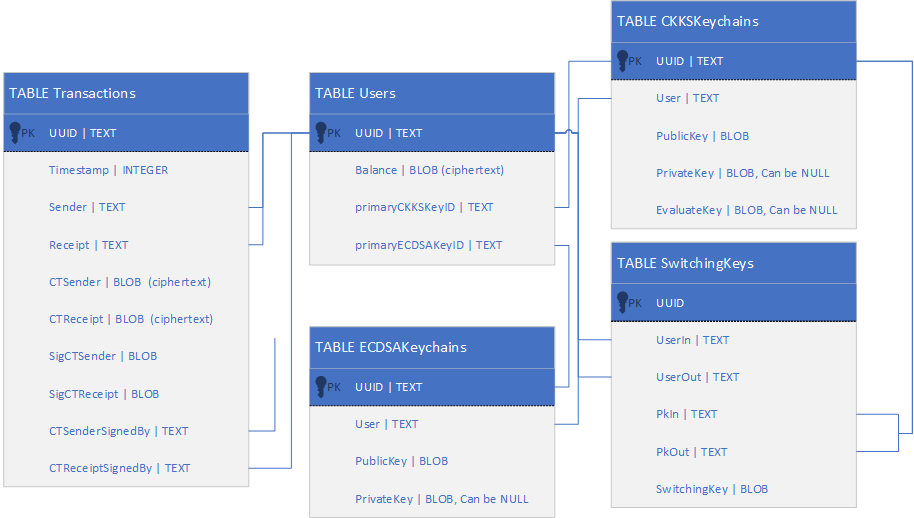
\includegraphics[width=\linewidth]{Figures/chimata-database-design.png}
    \caption{数据库设计示意图}\label{Fig:Database}
\end{figure}

在 Golang 中使用下面的语句导入 SQLite3 相关库:

\begin{minted}[frame=single]{go}
import (
    "database/sql" // 标准库
    
    database "github.com/CamberLoid/Chimata/internal/db" // 内部库
    _ "github.com/mattn/go-sqlite3" // 外部库,操作 SQLite3 数据库
)
\end{minted}

由于本文使用的数据库涉及到对外码的使用,使用了外码约束来保证数据库的一致性,因此在初始化数据库时需要额外添加指令:

\begin{minted}[frame=single]{go}
    db.Exec("PRAGMA foreign_keys = ON;")
\end{minted}
 
\subsection{交易信息}

结构体 \verb|Transaction| 包含在子包 \verb|internal/transaction| 内,被上层包所使用。其定义如下文所示

\begin{minted}[frame=single]{go}
type Transaction struct {
    ConfirmingPhase   string    `json:"confirmingPhase"`
    UUID              uuid.UUID `json:"uuid"`
    Sender            uuid.UUID `json:"sender"`
    Receipt           uuid.UUID `json:"receipt"`
    CTSender          []byte    `json:"ctSender"`
    CTReceipt         []byte    `json:"ctReceipt"`
    SigCTSender       []byte    `json:"sigCtSender"`
    CTSenderSignedBy  uuid.UUID `json:"ctSenderSignedBy"`
    SigCTReceipt      []byte    `json:"sigCTReceipt"`
    CTReceiptSignedBy uuid.UUID `json:"ctReceiptSignedBy"`
    TimeStamp         int64     `json:"timestamp"` //unix时间戳
    IsValid           bool      `json:"isValid"`
}    
\end{minted}

\begin{itemize}
    \item \verb|ConfirmingPhase|:交易的确认阶段,取值为 \verb|{"unconfirmed", "confirmed"|\\
    \verb|, "failed"}|,分别表示未确认、已确认和无效;
    \item \verb|Sender, Receipt|:作为外码标识交易的转出和转入方,其底层类型为 \verb|[16]byte|;
    \item \verb|CTSender, CTReceipt|:经过 \verb|rlwe.CipherText.MarshalBinary()| 方法反序列化的密文;
    \item \verb|SigCTSender, SigCTReceipt|:对密文的签名,由标准库 \verb|crypto/ecdsa| 中 \verb|ecdsa.SignASN1()| 产生;
\end{itemize}

该子包也包含了一些对交易信息的通用的辅助函数:

\begin{itemize}
    \item \verb|func (t Transaction) GetSenderCT() (ct *rlwe.Ciphertext, err error)|:输出序列化后的转出方密文;
    \item \verb|func (t Transaction) GetReceiptCT() (ct *rlwe.Ciphertext, err error)|:输出序列化后的转入方密文;
    \item \verb|func CalcFixedFee(ct *rlwe.Ciphertext, rate float64) *rlwe.Ciphertext|:计算固定费率的手续费;
    \item \verb|func CalcRatedFee(ct *rlwe.Ciphertext, rate float64) *rlwe.Ciphertext|:计算按比例费率的手续费;
\end{itemize}

\subsection{其他杂项:密钥链、用户和其他}

\subsubsection*{密钥链}

子包 \verb|internal/key| 定义了密钥链的相关结构体和函数,包括以下部分:

\begin{itemize}
    \item \verb|type CKKSKeyChain struct|:CKKS 方案所使用的密钥链结构体,包含了公钥对象的指针 \verb|CKKSPrivateKey *rlwe.SecretKey|,私钥钥对象的指针\\
    \verb|CKKSPublicKey *rlwe.PublicKey|,以及一个唯一标识符 \verb|Identifier uuid.UUID|
    \item \verb|type ECDSAKeyChain struct|:类似 CKKSKeyChain 的定义,此处不再赘述。
    \item \verb|type CKKSPayload interface|:包含了 \verb|MarshalBinary() ([]byte, error)| 和 \verb|UnmarshalBinary([]byte) error| 两个序列化和反序列化函数的接口,对应 lattigo 中的密文对象、公私钥对象和重加密密钥对象。
\end{itemize}

\subsubsection{用户}

子包 \verb|internal/user| 定义了基本的用户类型。代码声明如下:

\begin{minted}[frame=single]{go}
type User struct {
    UserIdentifier    uuid.UUID // 或者是 [16]bytes
    UserName          string
    UserCKKSKeyChain  []key.CKKSKeyChain
    UserECDSAKeyChain []key.ECDSAKeyChain
}
\end{minted}

\subsubsection{其他}

子包 \verb|internal/misc| 定义了一些其他的辅助函数,包括:

\begin{itemize}
    \item \verb|func NewCiphertext() *rlwe.Ciphertext|:创建新的空密文对象;
    \item \verb|func GenerateSwitchingKey(skIn, skOut *rlwe.SecretKey)|\\
    \verb|*rlwe.SwitchingKey|:将 lattigo 中的\verb|(...).GenSwitchingKey()| 进行封装的函数;
    \item \verb|func CKKSMsgRound(v float64) float64|:将由 CKKS 方案解密的浮点数,进行保留两位小数的四舍五入。
\end{itemize}

\section{客户端}

方案客户端实现以包 \verb|internal/clientlib| 提供,分为以下几个部分:

\begin{itemize}
    \item \verb|client.go|:包含 Client 对象及以其为接收器的高层级函数。\\
    一个 Client 对象包含了主用户的 UUID 和对应的数据库对象的指针。以 Client 为接收器,实现了转账请求函数、认可转账函数,以及获取交易信息中交易金额的函数。
    \item \verb|user.go|:包含了对 User 对象的定义和操作;\\
    此处 User 对象继承了 \verb|internal/user.User|,并实现了包括使用用户主密钥链签名,以及进行解密的函数。
    \item \verb|transaction.go|:以 User 对象为接收器,定义了交易相关的函数,包括了转账请求函数和认可转账函数的中层实现;
    \item \verb|server.go|:包含客户端与服务端的网络通信相关函数的文件;
    \item \verb|db.go|:包含客户端对数据库的初始化操作函数;
    \item \verb|crypto.go|:包含对 CKKS 方案中加密和解密函数的包装;
\end{itemize}

因精力有限,故本文不再附带客户端的 CLI\footnote{Command-Line Interface,命令行界面,常见于 Unix-like 系统中} 实现,仅提供该客户端库的集成测试函数,以进行实验和测试。测试过程和结果见下一章。

\subsection{客户端的主要函数}

本小节将对客户端被导出的主要函数进行简要介绍。

\subsubsection{密码学相关}

\begin{itemize}
    \item \verb|func CKKSEncryptAmount(float64, *rlwe.PublicKey) *rlwe.Ciphertext|:本文对 Lattigo 提供的加密函数的封装,以浮点数金额和公钥对象作为输入,输出密文对象的指针。
    \item \verb|func CKKSDecryptAmountFromCT(*rlwe.Ciphertext, *rlwe.SecretKey) float64 |:上述函数的反函数。
\end{itemize}

\subsubsection{网络通信相关}

\begin{itemize}
    \item \verb|func RegisterUser|:向服务端注册用户基本信息,包括 UUID、用户名、公钥链等;
    \item \verb|func RegisterSwk|:向服务端注册重加密密钥,也包括输入方和输出方的 UUID;
    \item \verb|func (*User) CreateTransferJob|:创建转账请求,方法包括对金额的加密、签名等;
    \item \verb|func (*User) GetBalance|:获取密文余额;
    \item \verb|func GetTransactionFromServer|:获取单笔交易的信息,其中交易金额为密文。
\end{itemize}

此外,在 \verb|server.go| 中还定义了变量 \verb|var ConfigServerURL string| 及其默认值,用于指定服务端的地址。

\section{服务端}

方案服务端实现以包 \verb|internal/serverlib| 和简单的程序实现 \verb|cmd/server| 提供。

\subsection{服务端主程序}

服务端中,其与客户端的通信经由 HTTP(S) 完成。对于每个暴露的 EndPoint,都有一个函数处理其接收的请求。服务端现阶段暴露的 EndPoints 如下:

\begin{itemize}
    \item \verb|/register/user|:注册用户基本信息的接口。若请求不合法则返回状态码 400\footnote{Bad Request},其他错误返回状态码 500\footnote{Internal Server Error,即服务端内部发生错误} 并包含错误描述,否则返回状态码 200 并中断连接;
    \item \verb|/register/swk|:向服务器提交重加密密钥的接口。若请求不合法则返回状态码 400,其他错误返回状态码 500 并包含错误描述,否则返回状态码 200 并中断连接;
    \item \verb|/transaction/create/bySenderPK| 和 \verb|/transaction/create/byReceiptPK|:创建转账请求的接口。当转账请求不合法时返回 HTTP 代码 400,签名验证失败返回状态码 401,其他错误返回状态码 500 并包含错误描述,否则返回状态码 200 并包含交易现阶段的所有信息;
    \item \verb|/transaction/confirm|:接收转账的接口,与上一条类似。
    \item \verb|/transaction/get|:获取交易信息的接口。该接口不需要鉴权。若请求不合法则返回状态码 400,其他错误返回状态码 500 并包含错误描述,否则返回状态码 200 并包含交易现阶段的所有信息;
    \item \verb|/user/GetBalance|:获取密文余额的接口。若请求不合法则返回状态码 400,其他错误返回状态码 500 并包含错误描述,否则返回状态码 200 并包含用户的密文余额;
\end{itemize}

主函数如下:

\begin{minted}[frame=single]{go}
func main(){
    loggerInit()
    http.HandleFunc("/transaction/create/bySenderPK", 
        HandlerTransactionCreateBySenderPK)
    // ... 忽略其他接口声明
    
    // 打开数据库
    if Database, err = InitDatabase(); err != nil {
        CriticalLogger.Fatal(err.Error())
    }
    defer Database.Close()

    // 开始监听
    InfoLogger.Printf("Listening: %v", 
        ConfigListenAddr+":"+ConfigListenPort)
    if err := http.ListenAndServe(
        ConfigListenAddr+":"+ConfigListenPort,
        nil); err != nil {
        log.Fatal(err)
    }
}
\end{minted}

\subsection{服务端库 serverlib}

服务端库 \verb|serverlib| 中包含了服务端的主要逻辑,包括对数据库的操作、对交易的处理、对用户的处理等。包括的重点函数和结构体如下:

\begin{itemize}
    \item \verb|func ReEncryptCTWithSwk(ct, swk)|:调用 \verb|evaluator.SwitchKeysNew| 方法,对密文进行重加密。同时也包含处理重加密失败时将 panic 转换为错误 error 的逻辑。
    \item \verb|func KeySwitchSenderToReceipt| 与 \verb|func KeySwitchReceiptToSender|:这两个方法从更高的层级,调用上述 \verb|ReEncryptCTWithSwk()|。
    \item \verb|func ValidateSignatureForCipherText(ct interface{}, sig []byte,|\\ 
    \verb|pk *ecdsa.PublicKey)|:对密文的签名进行验证,包含处理不同种类密文,即密文对象和/或密文反序列化后的字节流的逻辑。
    \item \verb|func GetUpdatedBalance|:对交易后的账户进行处理的逻辑,包括对密文余额的更新。
    \item \verb|func InitializeNewReceiptPKTransaction|、\\
    \verb|func InitializeNewSenderPKTransaction| 和 \verb|func FinishTransaction|:处理交易信息的支援性函数
    \item \verb|type User struct|:该类型继承了 \verb|users.User|,并多一个 Balance 对象。
\end{itemize}
